\section{运行模型}
\label{sec:exec-model}

\begin{frame}
  \begin{center}
    \Huge{\textcolor{red}{运行模型}}
  \end{center}

  \begin{enumerate}
    \item \alert{运行模式}
    \item \alert{创建会话}
    \item \alert{RunStep过程}
  \end{enumerate}
\end{frame}

\subsection{运行模式}

\begin{frame}{本地模式}
  \begin{figure}
    \centering
    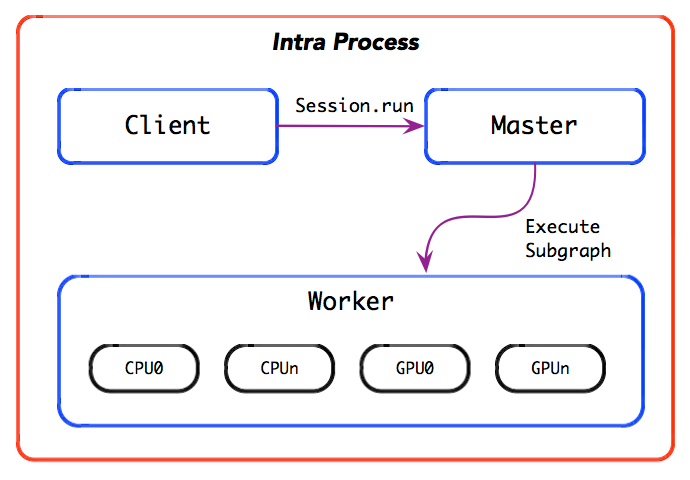
\includegraphics[width=0.6\textwidth]{local.png}
  \end{figure}
\end{frame}

\begin{frame}{分布式模式}
  \begin{figure}
    \centering
    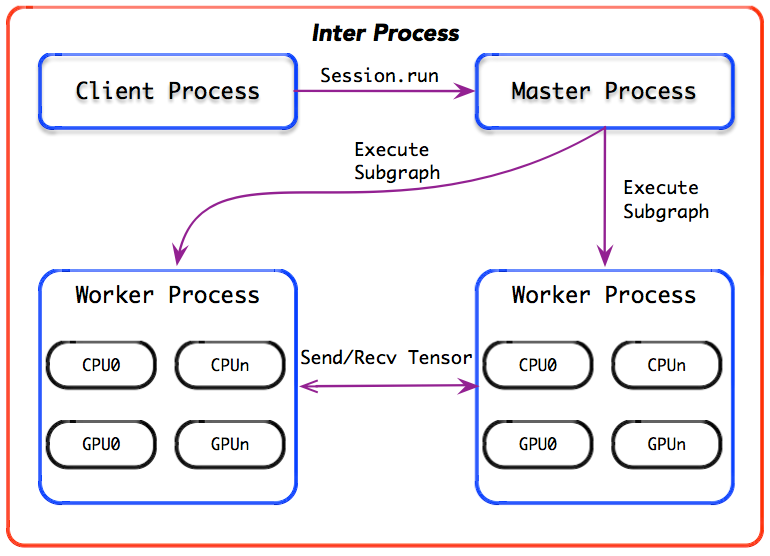
\includegraphics[width=0.6\textwidth]{distributed.png}
  \end{figure}
\end{frame}

\subsection{创建会话}

\begin{frame}{创建ClientSession}
  \begin{figure}
    \centering
    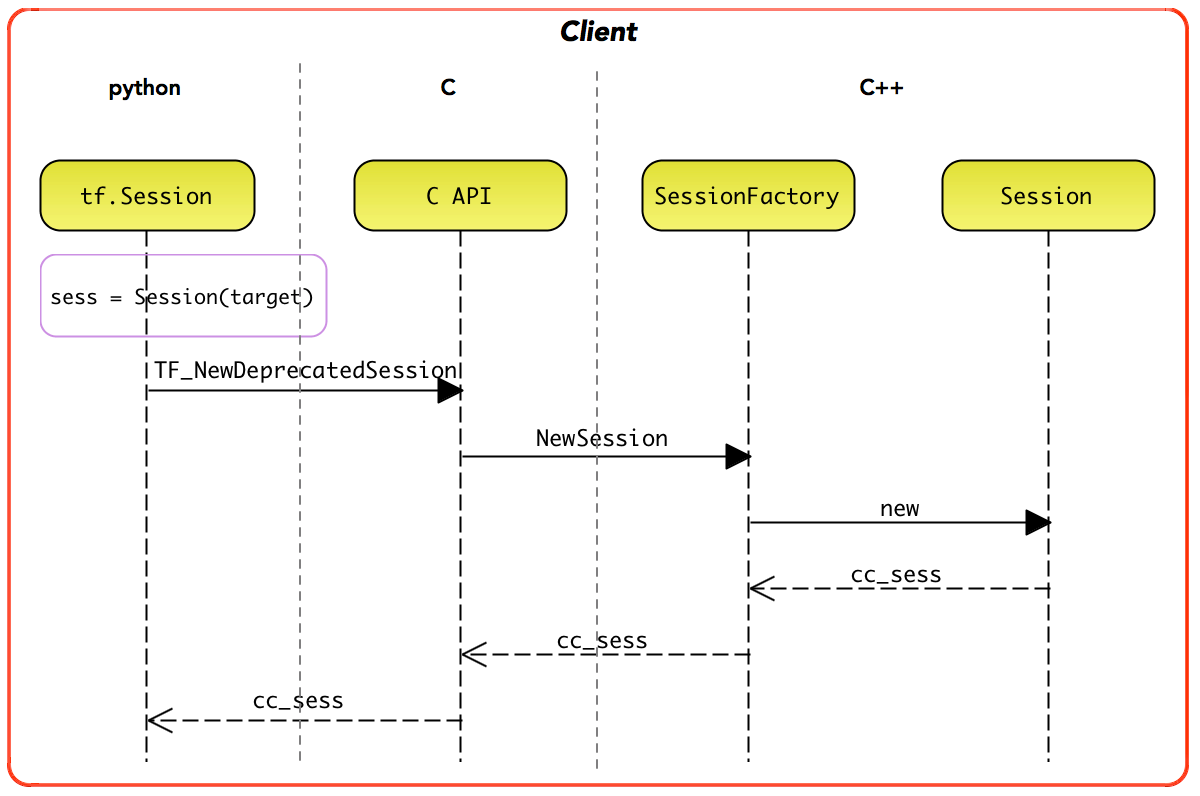
\includegraphics[width=0.8\textwidth]{cc-client-session.png}
  \end{figure}
\end{frame}

\begin{frame}{多态创建}
  \begin{figure}
    \centering
    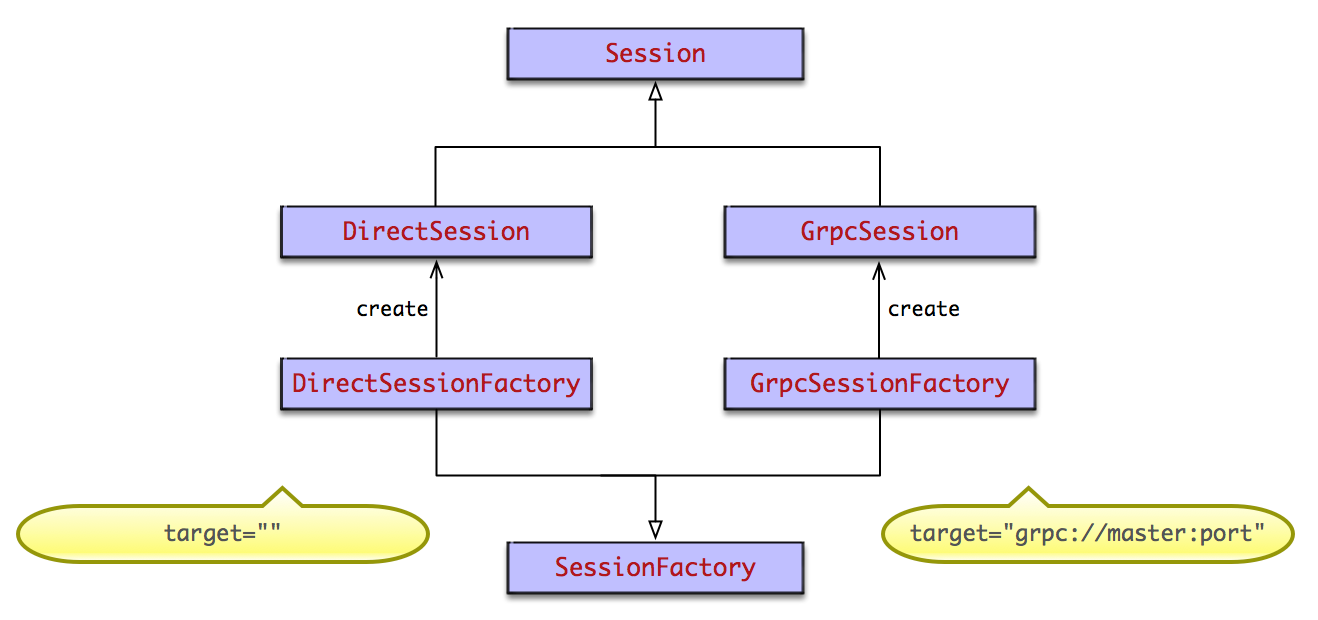
\includegraphics[width=1.0\textwidth]{cc-session-factory.png}
  \end{figure}
\end{frame}

\begin{frame}{创建MasterSession}
  \begin{figure}
    \centering
    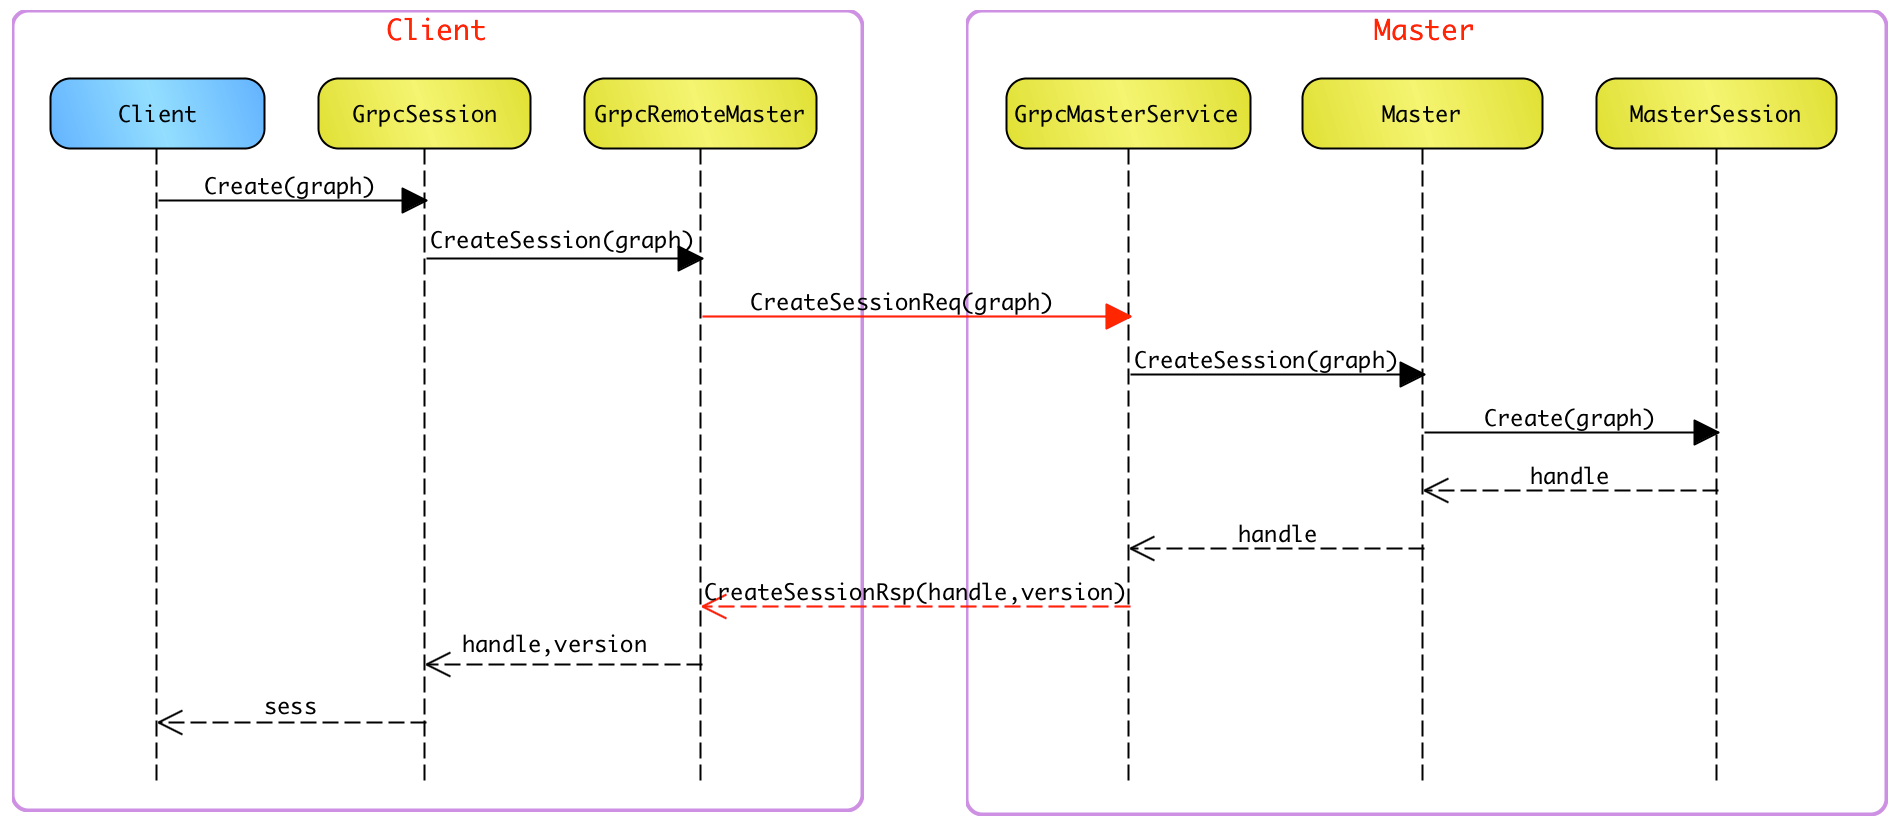
\includegraphics[width=1.0\textwidth]{cc-create-master-session.png}
  \end{figure}
\end{frame}

\begin{frame}{MasterSession模型}
  \begin{figure}
    \centering
    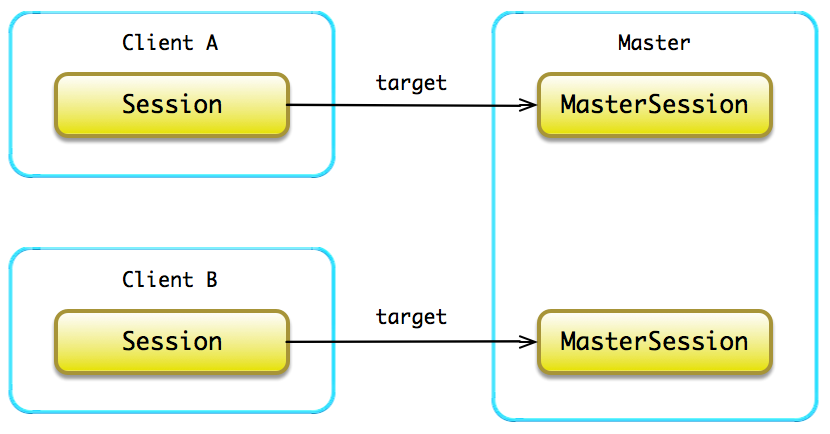
\includegraphics[width=0.8\textwidth]{cc-create-master-session-model.png}
  \end{figure}
\end{frame}

\subsection{RunStep过程}

\begin{frame}{一级图分裂}
  \begin{figure}
    \centering
    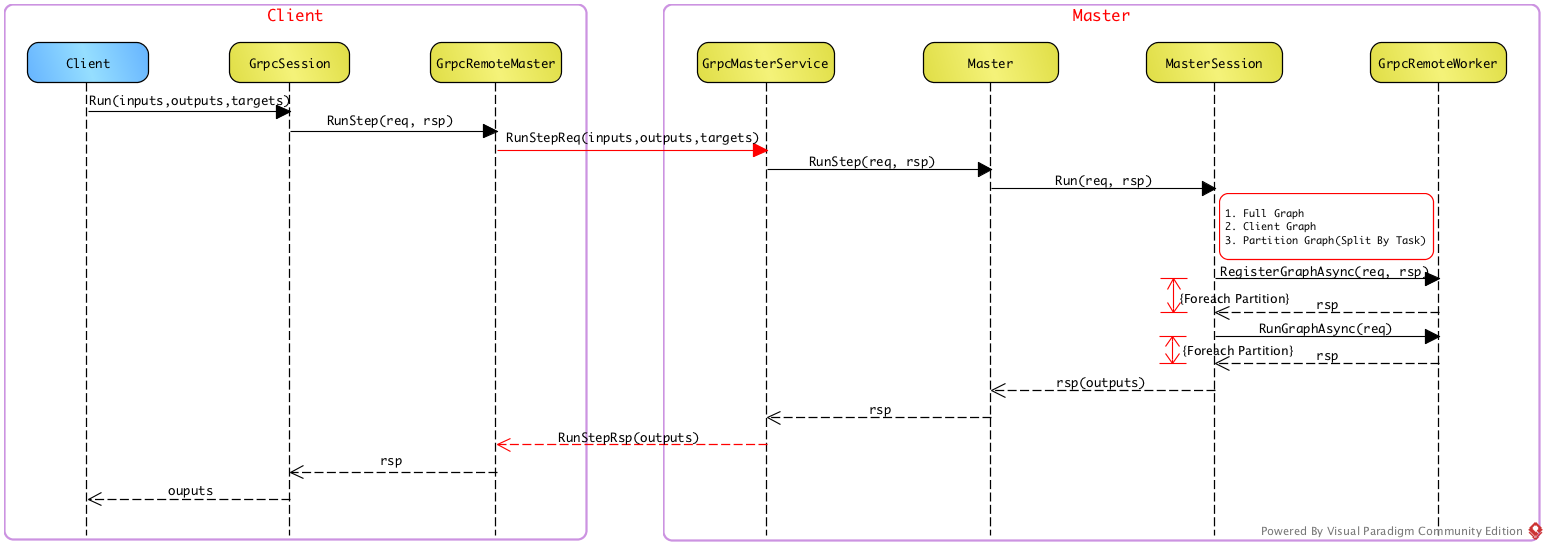
\includegraphics[width=1.0\textwidth]{cc-run-step-client-to-master.png}
  \end{figure}
\end{frame}

\begin{frame}{二级图分裂}
  \begin{figure}
    \centering
    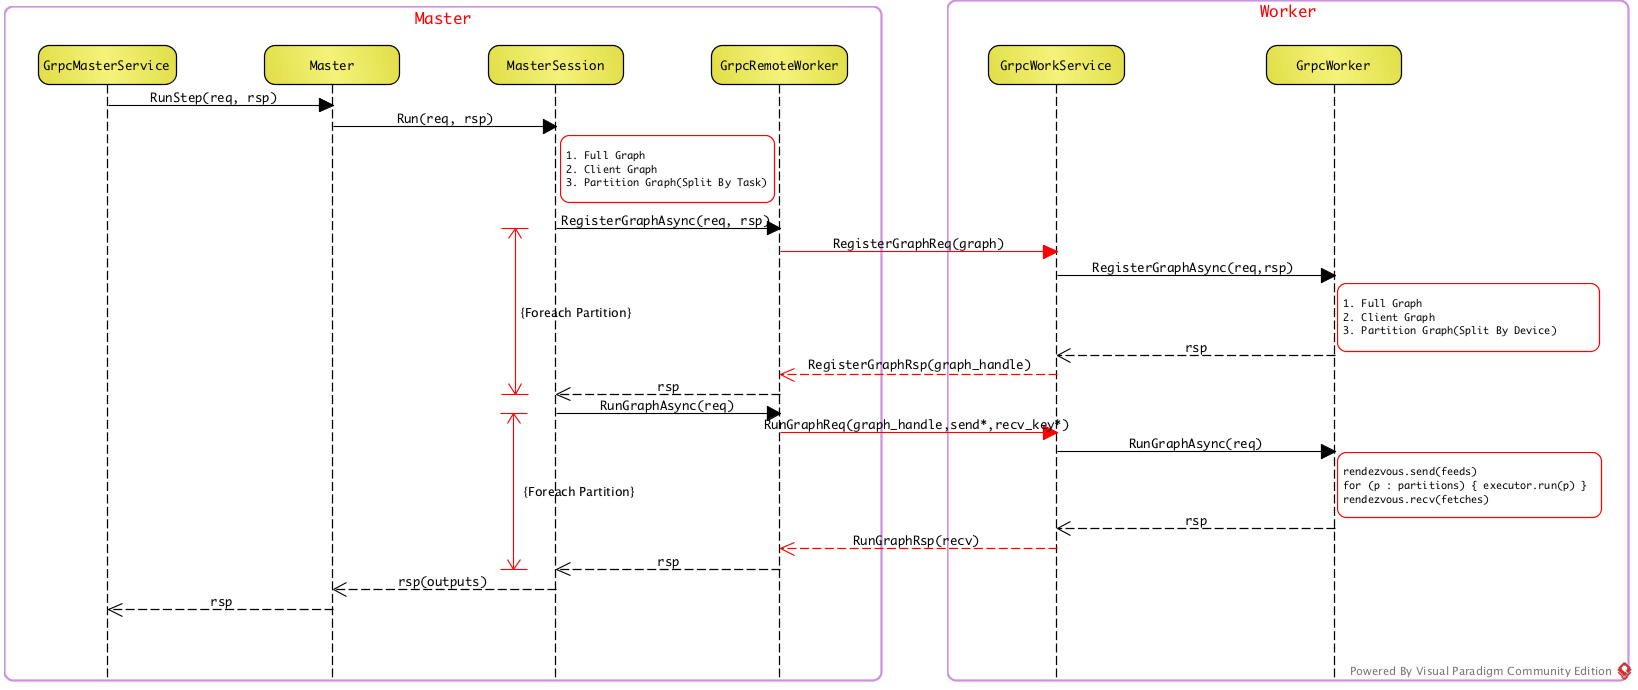
\includegraphics[width=1.0\textwidth]{cc-run-step-master-to-worker.png}
  \end{figure}
\end{frame}

\begin{frame}{实例:图分裂}
  \begin{figure}
    \centering
    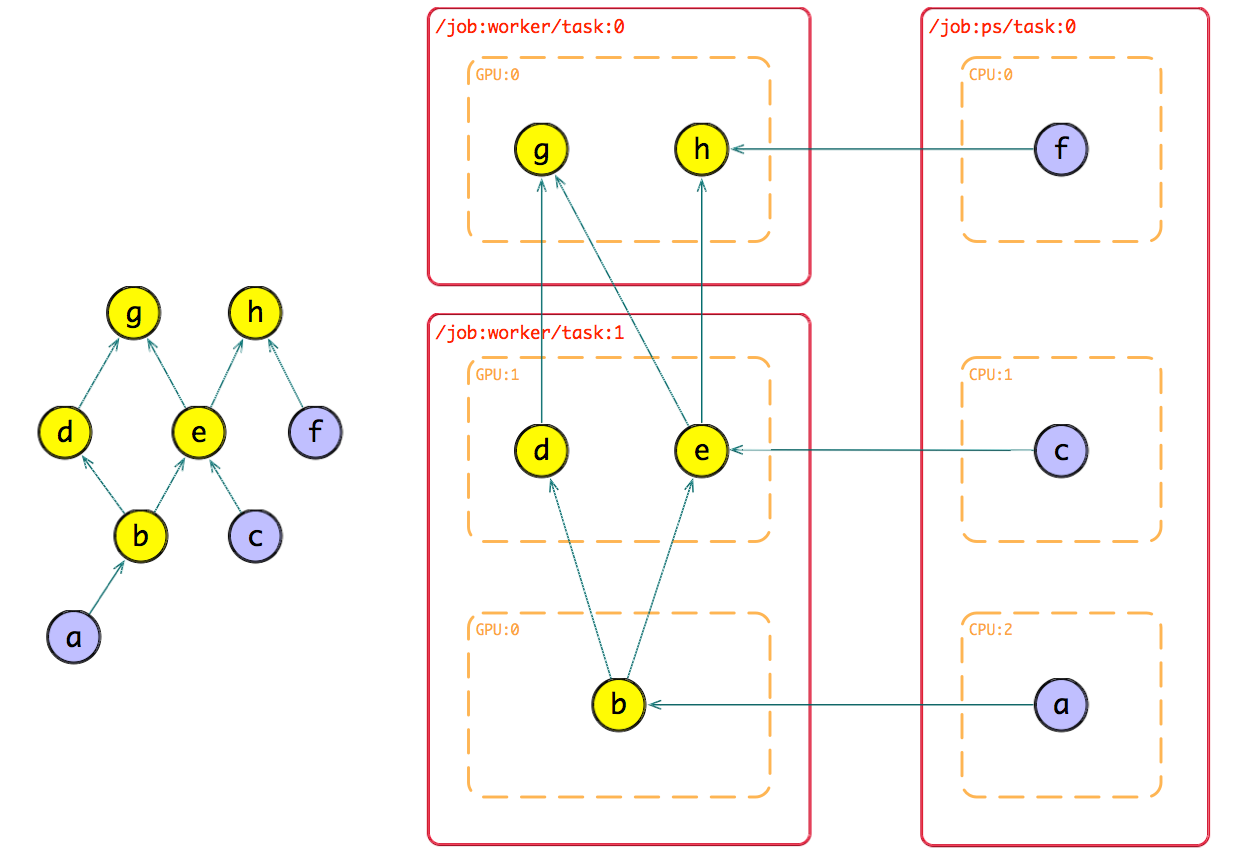
\includegraphics[width=0.79\textwidth]{cc-dist-graph-split-by-task-exam-1.png}
  \end{figure}
\end{frame}

\begin{frame}{实例:交换数据}
  \begin{figure}
    \centering
    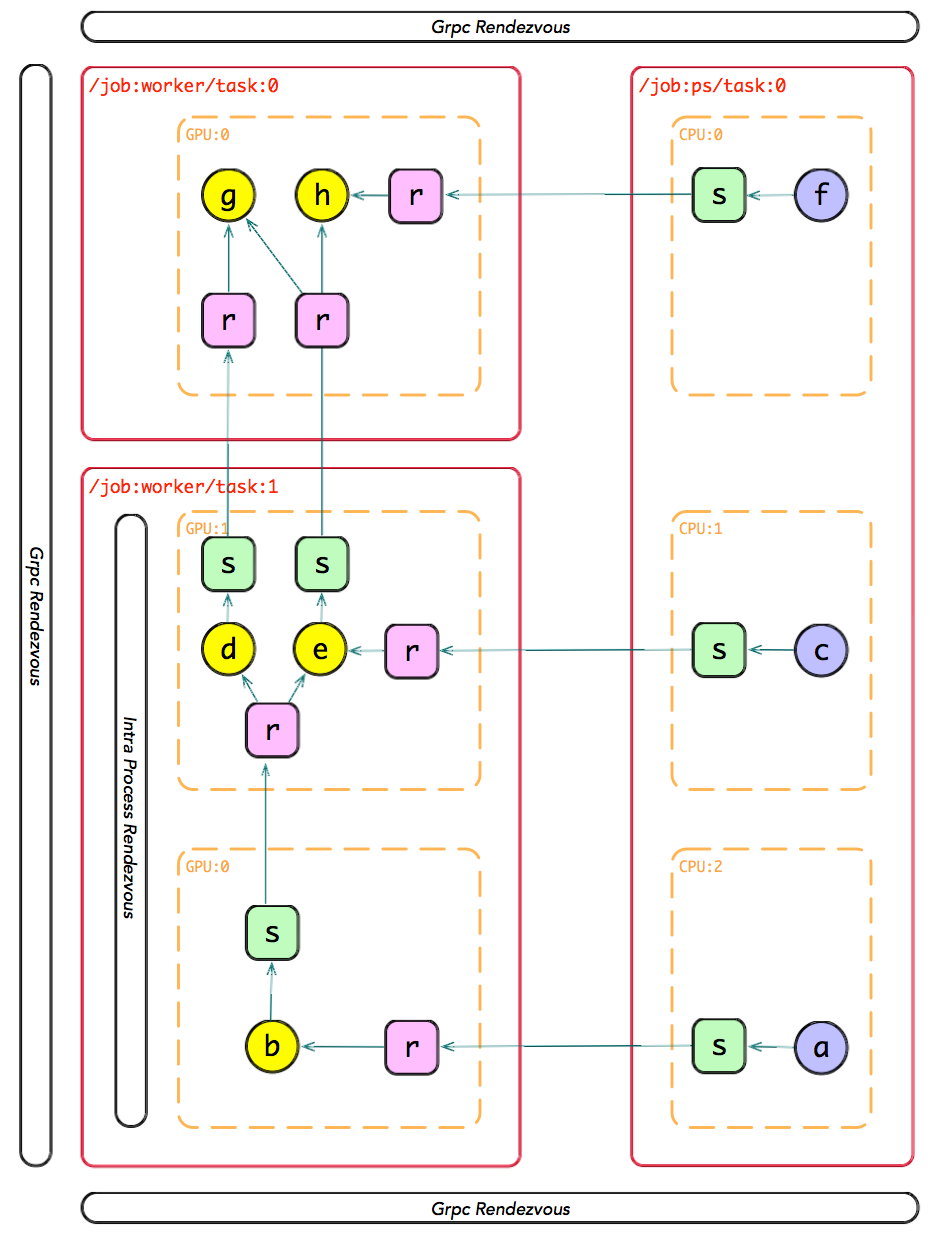
\includegraphics[width=0.45\textwidth]{cc-dist-graph-split-by-task-exam-2.png}
  \end{figure}
\end{frame}